
\begin{figure}[H]
\centering
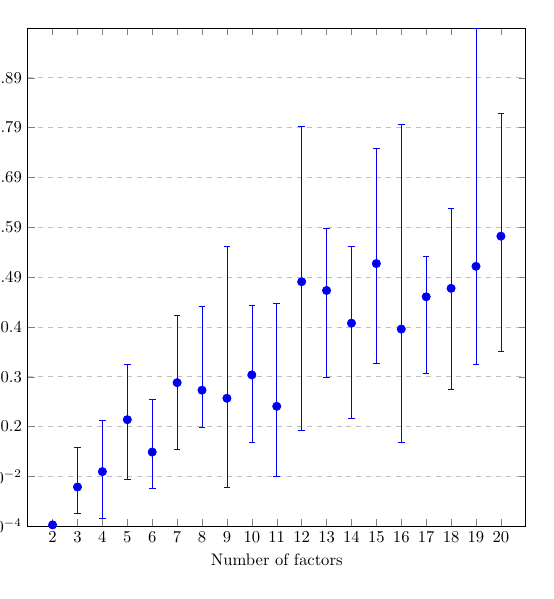
\begin{tikzpicture}[scale=0.6, trim axis left, trim axis right]
\begin{axis}[
    width=1\textwidth,
    height=1\textwidth,
    xlabel={Number of factors},
    ylabel={Time taken (s)},
    xmin=1.0, xmax=21.0,
    ymin=0.000164, ymax=0.988235,
    xticklabels={2, 3, 4, 5, 6, 7, 8, 9, 10, 11, 12, 13, 14, 15, 16, 17, 18, 19, 20},
    xtick={2, 3, 4, 5, 6, 7, 8, 9, 10, 11, 12, 13, 14, 15, 16, 17, 18, 19, 20},
    ytick={0.000164, 0.0989711, 0.1977782, 0.2965853, 0.3953924, 0.4941995, 0.5930066, 0.6918137, 0.7906208, 0.8894279},
    ymajorgrids=true,
    grid style=dashed,
]

\addplot+[
    blue,
    very thick,
    forget plot,
    only marks
    ]
    plot[
    very thick,
    error bars/.cd,
    y dir=plus,
    y explicit
    ]
    table[x=x,y=y,y error expr=\thisrow{y-max}] {
    x    y    y-max
    11	0.2378325	0.2036185
10	0.3001564	0.1381466
13	0.4676492	0.1223558
12	0.4849881	0.3092019
15	0.5210108	0.2293392
14	0.4027823	0.1531237
17	0.4551362	0.0797818
16	0.3910601	0.4061569
19	0.5155398	0.4726952
18	0.4719107	0.1577003
20	0.5753437	0.2442193
3	0.077821	0.078674
2	0.0026672	0.0039028
5	0.2113494	0.1107546
4	0.1083478	0.1015632
7	0.2847528	0.1333312
6	0.1471398	0.1046092
9	0.2538288	0.3020072
8	0.2698269	0.1655141

    };

\addplot+[
    blue,
    very thick,
    forget plot,
    only marks
    ]
    plot[
    very thick,
    error bars/.cd,
    y dir=plus,
    y explicit
    ]
    table[x=x,y=y,y error expr=\thisrow{y-min}] {
    x    y    y-min
    11	0.2378325	-0.1395065
10	0.3001564	-0.1329344
13	0.4676492	-0.1713402
12	0.4849881	-0.2946451
15	0.5210108	-0.1970208
14	0.4027823	-0.1886093
17	0.4551362	-0.1526042
16	0.3910601	-0.2246801
19	0.5155398	-0.1938318
18	0.4719107	-0.2005797
20	0.5753437	-0.2279057
3	0.077821	-0.052674
2	0.0026672	-0.0025032
5	0.2113494	-0.1183274
4	0.1083478	-0.0934608
7	0.2847528	-0.1318138
6	0.1471398	-0.0722868
9	0.2538288	-0.1763108
8	0.2698269	-0.0745989

    };

\end{axis}
\end{tikzpicture}
\vspace{-0.3cm}
\caption{LenstrasEllipticCurveFactorization Medium primes}\label{fig:LenstrasEllipticCurveFactorizationmediumprimes(maximumIterations:-1)factors}
\end{figure}
